\documentclass[11pt,a4paper]{ctexart}
\usepackage[student]{ipara}
\tcbuselibrary{skins,breakable}
\usepackage{multicol}
\usepackage{longtable}
\usepackage{tikz}
\usepackage{tikz-3dplot}
\usetikzlibrary{shapes.geometric, arrows.meta, positioning, calc}
\usepackage{amsthm}

% =====================================================
% 重复引入防重载保护 (Input Guard)
% =====================================================
\makeatletter
\newcommand{\loadedfiles}{}
\let\oldinput\input
\renewcommand{\input}[1]{%
  \edef\temp@args{{#1}{\loadedfiles}}%
  \expandafter\check@loaded\temp@args
  \ifin@
  \else
    \g@addto@macro\loadedfiles{#1,}%
    \oldinput{#1}%
  \fi
}
\newcommand{\check@loaded}[2]{\in@{#1}{#2}}
\makeatother

% =====================================================
% TikZ 几何直观图示宏包（高清黑白印刷级）
% =====================================================
\newcommand{\sineLawFigure}{%
  \begin{center}
    \begin{tikzpicture}[scale=0.88, line join=round, line cap=round]
      \coordinate (O) at (0,0);
      \coordinate (A) at (210:2.0);
      \coordinate (B) at (330:2.0);
      \coordinate (C) at (80:2.0);
      \draw[gray!65, thick] (O) circle (2.0);
      \draw[very thick] (A)--(B)--(C)--cycle;
      \draw[dashed, gray!70] (O)--(A) (O)--(B) (O)--(C);
      \fill (O) circle (1.2pt) node[right] {\small \(O\)};
      \foreach \p/\pos in {A/below left,B/below right,C/above} {
        \fill (\p) circle (1.2pt) node[\pos] {\small \(\p\)};
      }
      \node[below] at ($(A)!0.5!(B)$) {\small \(c\)};
      \node[right] at ($(B)!0.5!(C)$) {\small \(a\)};
      \node[left] at ($(C)!0.5!(A)$) {\small \(b\)};
      \node at (0,-2.35) {\small\textbf{图 1 外接圆半径 \(R\) 与正弦定理}};
    \end{tikzpicture}
  \end{center}
}

\newcommand{\cosineLawFigure}{%
  \begin{center}
    \begin{tikzpicture}[scale=0.92, line join=round, line cap=round]
      \coordinate (A) at (0,0);
      \coordinate (B) at (3.2,0);
      \coordinate (C) at (0.9,1.65);
      \draw[very thick] (A)--(B)--(C)--cycle;
      \node[below] at (A) {\small \(A\)};
      \node[below] at (B) {\small \(B\)};
      \node[above] at (C) {\small \(C\)};
      \node[below] at ($(A)!0.5!(B)$) {\small \(c\)};
      \node[right] at ($(B)!0.5!(C)$) {\small \(a\)};
      \node[left] at ($(C)!0.5!(A)$) {\small \(b\)};
      \draw[->] (A) +(0.55,0) arc[start angle=0,end angle=61,radius=0.55];
      \node at (0.66,0.27) {\small \(A\)};
      \node at (1.6,-0.4) {\small\textbf{图 2 余弦定理三边一角关系}};
    \end{tikzpicture}
  \end{center}
}

\newcommand{\freedomFigure}{%
  \begin{center}
    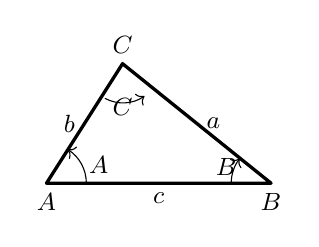
\begin{tikzpicture}[scale=0.92, line join=round, line cap=round]
      \coordinate (A) at (0,0);
      \coordinate (B) at (3.1,0);
      \coordinate (C) at (1.05,1.65);
      \draw[very thick] (A)--(B)--(C)--cycle;
      \node[below] at (A) {\small \(A\)};
      \node[below] at (B) {\small \(B\)};
      \node[above] at (C) {\small \(C\)};
      \node[below] at ($(A)!0.5!(B)$) {\small \(c\)};
      \node[right] at ($(B)!0.5!(C)$) {\small \(a\)};
      \node[left] at ($(C)!0.5!(A)$) {\small \(b\)};
      \draw[->] (A) +(0.55,0) arc[start angle=0,end angle=58,radius=0.55];
      \draw[->] (B) +(-0.55,0) arc[start angle=180,end angle=142,radius=0.55];
      \draw[->] (C) +(-0.24,-0.48) arc[start angle=242,end angle=305,radius=0.52];
      \node at (0.72,0.25) {\small \(A\)};
      \node at (2.48,0.22) {\small \(B\)};
      \node at (1.05,1.05) {\small \(C\)};
    \end{tikzpicture}
  \end{center}
}

\newcommand{\axisSphereModelFigure}{%
  \begin{center}
    \begin{tikzpicture}[scale=1.0, >=stealth, line join=round, line cap=round]
      \coordinate (O) at (0,0);
      \coordinate (T) at (0,1.0);
      \coordinate (P) at (1.55,1.0);
      \draw[thick] (O) circle (1.85);
      \draw[thick] (-1.55,1.0) arc (180:360:1.55 and 0.28);
      \draw[dashed] (1.55,1.0) arc (0:180:1.55 and 0.28);
      \draw[thick] (-1.55,-1.0) arc (180:360:1.55 and 0.28);
      \draw[dashed] (1.55,-1.0) arc (0:180:1.55 and 0.28);
      \draw[thick] (-1.55,1.0) -- (-1.55,-1.0);
      \draw[thick] (1.55,1.0) -- (1.55,-1.0);
      \draw[dashed, semithick, gray] (O) -- (T);
      \draw[dashed, semithick, gray] (T) -- (P);
      \draw[dashed, semithick, gray] (O) -- (P);
      \draw[thin] (T) ++(0.18,0) -- ++(0, -0.18) -- ++(-0.18,0);
      \fill (O) circle (1.2pt) node[left] {\small $O$};
      \fill (T) circle (1.1pt) node[left] {\small $O_1$};
      \fill (P) circle (1.1pt);
      \node[left] at ($(O)!0.5!(T)$) {\small $d$};
      \node[above] at ($(T)!0.5!(P)$) {\small $r$};
      \node[right] at ($(O)!0.5!(P)$) {\small $R$};
      \node[below] at (0,-2.15) {\small\textbf{图 3 核心轴心截面：$R^2=r^2+d^2$}};
    \end{tikzpicture}
  \end{center}
}

\newcommand{\insphereVolumeFigure}{%
  \begin{center}
    \begin{tikzpicture}[scale=0.95, >=stealth, line join=round, line cap=round]
      \coordinate (P) at (0,2.0);
      \coordinate (A) at (-1.7,-0.6);
      \coordinate (B) at (1.7,-0.6);
      \coordinate (C) at (0.55,0.35);
      \coordinate (O) at (0,0.15);
      \draw[dashed, thick, gray!75] (A) -- (C) -- (B);
      \draw[thick] (P) -- (A) -- (B) -- cycle;
      \draw[thick] (P) -- (C);
      \draw[gray, thick] (O) circle (0.42);
      \draw[dashed, gray] (O) -- (-0.45,0.65);
      \node[right] at (O) {\small $O$};
      \node[left] at (-0.42,0.52) {\small $r$};
      \node[above] at (P) {\small $P$};
      \node[left] at (A) {\small $A$};
      \node[below] at (B) {\small $B$};
      \node[right] at (C) {\small $C$};
      \node[below] at (0,-1.0) {\small\textbf{图 4 内切球等体积法：$V=\frac13S_{\text{表}}r$}};
    \end{tikzpicture}
  \end{center}
}

\newcommand{\reviewMapFigure}{%
  \begin{center}
    \begin{tikzpicture}[>=stealth, line join=round, line cap=round]
      \node[draw, thick, rounded corners=1mm, minimum width=2.7cm, minimum height=0.8cm] (A) at (0,0) {\small 识别图形};
      \node[draw, thick, rounded corners=1mm, minimum width=2.7cm, minimum height=0.8cm] (B) at (3.4,0) {\small 确定点线面};
      \node[draw, thick, rounded corners=1mm, minimum width=2.7cm, minimum height=0.8cm] (C) at (6.8,0) {\small 找平行垂直};
      \node[draw, thick, rounded corners=1mm, minimum width=2.7cm, minimum height=0.8cm] (D) at (1.7,-1.35) {\small 转化到平面};
      \node[draw, thick, rounded corners=1mm, minimum width=2.7cm, minimum height=0.8cm] (E) at (5.1,-1.35) {\small 建系计算};
      \draw[->, thick] (A) -- (B);
      \draw[->, thick] (B) -- (C);
      \draw[->, thick] (B) -- (D);
      \draw[->, thick] (C) -- (E);
      \draw[->, thick] (D) -- (E);
    \end{tikzpicture}
  \end{center}
}

% =====================================================
% 页眉页脚高级配置 (结合 zref-lastpage)
% =====================================================
\pagestyle{fancy}
\fancyhf{}
\lhead{\small\color{black!70}\textbf{高中数学核心方法与典型例题解析 · 学生手册}}
\rhead{\small\color{black!70}\leftmark}
\cfoot{\small 第 \thepage\ 页\quad 共 \zpageref{LastPage} 页}
\renewcommand{\headrulewidth}{0.4pt}
\renewcommand{\footrulewidth}{0pt}

% =====================================================
% 引入公共题库试题
% =====================================================
% =====================================================
% 题型：双曲线离心率填空题 (q_hyperbola_eccentricity.tex)
% 知识板块：双曲线
% 主思维：定义优先思维
% 副思维：公式结构
% 错因标签：标准式化简错误、a, b, c 方程记混
% 讲义用途：圆锥曲线基础
% =====================================================
% 难度：★ (基础)
% =====================================================
\newcommand{\qHyperbolaEccentricityStem}{双曲线 \(5x^2 - 6y^2 = 1\) 的离心率为 \blank{3cm}。}

\newcommand{\qHyperbolaEccentricityAnswer}{\(\sqrt{\dfrac{11}{6}}\)}

\newcommand{\qHyperbolaEccentricitySolution}{%
  \textbf{【解题思路】}\par
  求双曲线的离心率，核心在于将一般式方程化为标准形式 \(\dfrac{x^2}{a^2} - \dfrac{y^2}{b^2} = 1\)，进而读取参数 \(a^2, b^2\)，结合恒等式 \(c^2 = a^2 + b^2\) 求得焦距 \(c\)，最终由离心率定义 \(e = \dfrac{c}{a}\) 求解。\par\vspace{0.4em}

  \textbf{【解析计算】}\par
  已知双曲线方程为 \(5x^2 - 6y^2 = 1\)，将其化为标准形式：
  \[
    \frac{x^2}{\frac{1}{5}} - \frac{y^2}{\frac{1}{6}} = 1.
  \]
  由此可得焦点在 \(x\) 轴上，且参数为：
  \[
    a^2 = \frac{1}{5}, \qquad b^2 = \frac{1}{6}.
  \]
  在双曲线中，焦距平方满足关系式：
  \[
    c^2 = a^2 + b^2 = \frac{1}{5} + \frac{1}{6} = \frac{11}{30}.
  \]
  由离心率定义公式，可得：
  \[
    \begin{aligned}
      e^2 &= \frac{c^2}{a^2} = \frac{\frac{11}{30}}{\frac{1}{5}} = \frac{11}{6} \\[0.4em]
      \implies e &= \sqrt{\frac{11}{6}} \quad \text{（或化简为 } \frac{\sqrt{66}}{6}\text{）}.
    \end{aligned}
  \]
  故答案为 \(\sqrt{\dfrac{11}{6}}\)。%
}

\newcommand{\qHyperbolaEccentricityDiagnosis}{%
  学生在化简方程时，容易将 \(5x^2\) 变形错误（如错记为 \(a^2 = 5\)）。同时，双曲线的几何性质中 \(c^2 = a^2 + b^2\) 极易与椭圆的 \(c^2 = a^2 - b^2\) 记混。%
}

\newcommand{\qHyperbolaEccentricityTeachingNotes}{%
  离心率计算是圆锥曲线的基础考点。讲评时应重点强化两点：一是“化标准”，将二次项系数化为 1 后，分母即为对应的平方项；二是区分椭圆与双曲线的 \(a, b, c\) 方程关系，夯实基础。%
}

% =====================================================
% 题型：函数最值与参数范围选择题 (q_func_max_val_parameter.tex)
% 知识板块：导数、最值
% 主思维：最值模型分析
% 副思维：函数思维、边界与端点检验、充分必要
% 错因标签：只证最大值小于等于1，忽略存在点取等
% 讲义用途：恒成立/最值系列
% =====================================================
% 难度：★★ (中档)
% =====================================================
\newcommand{\qFuncMaxValParameterStem}{已知函数 \(f(x) = \dfrac{x + 2}{e^x + a}\) 的最大值为 \(1\)，则 \(a = \hfill （\quad）\)}

\newcommand{\qFuncMaxValParameterOptions}{%
  \mcoptions[4]{\(\dfrac{1}{2}\)}{\(1\)}{\(\dfrac{3}{2}\)}{\(2\)}%
}

\newcommand{\qFuncMaxValParameterAnswer}{B}

\newcommand{\qFuncMaxValParameterSolution}{%
  \textbf{【解题思路】}\par
  本题为导数求最值与确定参数的综合应用题。第一步，求出函数 \(f(x)\) 的导数；第二步，利用“若可导函数在 \(x = x_0\) 处取得极值/最值，则必有 \(f'(x_0) = 0\)”，联立最值条件 \(f(x_0) = 1\) 与极值条件 \(f'(x_0) = 0\)，消去参数 \(a\) 求得极值点 \(x_0\)；第三步，回代求得 \(a\) 并验证极值点。\par\vspace{0.4em}

  \textbf{【解析计算】}\par
  已知函数为 \(f(x) = \dfrac{x + 2}{e^x + a}\)，对其求导得：
  \[
    \begin{aligned}
      f'(x) &= \frac{(e^x + a) - (x + 2)e^x}{(e^x + a)^2} \\[0.4em]
            &= \frac{a - (x + 1)e^x}{(e^x + a)^2}.
    \end{aligned}
  \]
  设函数在 \(x = x_0\) 处取得最大值 \(1\)，则同时满足极值与最值条件：
  \begin{enumerate}[leftmargin=2em, itemsep=0.3em, topsep=0.3em]
    \item 极值点导数为 \(0\)：
      \[
        f'(x_0) = 0 \implies a = (x_0 + 1)e^{x_0};
      \]
    \item 最大值为 \(1\)：
      \[
        f(x_0) = 1 \implies \frac{x_0 + 2}{e^{x_0} + a} = 1 \implies a = x_0 + 2 - e^{x_0}.
      \]
  \end{enumerate}
  联立两式消去参数 \(a\)，可得：
  \[
    \begin{aligned}
      (x_0 + 1)e^{x_0} &= x_0 + 2 - e^{x_0} \\[0.3em]
      \implies (x_0 + 2)e^{x_0} &= x_0 + 2 \\[0.3em]
      \implies (x_0 + 2)(e^{x_0} - 1) &= 0.
    \end{aligned}
  \]
  解得：\(x_0 = -2\) 或 \(x_0 = 0\)。\par\vspace{0.3em}

  \begin{enumerate}[leftmargin=2em, label=(\arabic*), itemsep=0.3em, topsep=0.3em]
    \item 若 \(x_0 = -2\)，代入求得 \(a = (-2 + 1)e^{-2} = -e^{-2} < 0\)，此时分母在某处可能为零且与选项不符，舍去；
    \item 若 \(x_0 = 0\)，代入求得 \(a = (0 + 1)e^0 = 1\)。
  \end{enumerate}

  当 \(a = 1\) 时，分母 \(e^x + 1 > 0\) 恒成立，验证知 \(f(x)\) 在 \(x = 0\) 处确实取得最大值 \(1\)。\par\vspace{0.2em}

  故选 \textbf{B}。%
}

\newcommand{\qFuncMaxValParameterDiagnosis}{%
  学生在对商的求导法则进行计算时容易出现符号混乱，特别是在合并分子时漏掉括号。此外，部分学生面对两个方程联立时可能感到无从下手，需要掌握消元（消去参数 \(a\)）的解题策略。特别要注意，“最大值为1”蕴含充分与必要两个方面，不仅要求函数值小于等于1，还必须保证有取等点。%
}

\newcommand{\qFuncMaxValParameterTeachingNotes}{%
  本题是一道精妙的导数选填题。解题突破口在于“最值点”的双重性质——即函数值等于最值，且在该点导数（极值点）为 0。联立消元是常见的代数变形技巧，讲评时应重点拆解这一联立过程。%
}

% =====================================================
% 题型：三圆共截线与弦长最值多项选择题 (q_conic_circle_chords.tex)
% 知识板块：圆与直线
% 主思维：数形结合与几何直观
% 副思维：最值模型分析、分类讨论、边界
% 错因标签：弦长公式不会转距离、相切临界条件遗漏
% 讲义用途：解析几何图像题
% =====================================================
% 难度：★★★ (难题)
% =====================================================
\newcommand{\qConicCircleChordsStem}{已知圆 \(C_1: (x + 1)^2 + y^2 = 1\)，圆 \(C_2: (x - 1)^2 + y^2 = 1\)，圆 \(C_3: x^2 + (y - \sqrt{3})^2 = 1\)，直线 \(l: y = kx + b\) 与 \(C_1, C_2, C_3\) 均有两个交点。记 \(l\) 被 \(C_1, C_2, C_3\) 截得的弦长分别为 \(s_1, s_2, s_3\)，则 \hfill （\quad）}

\newcommand{\qConicCircleChordsOptions}{%
  \mcoptions[2]{\(k\) 可以取任意实数}{\(满足\ s_1 = s_2 = s_3\) 的直线共有 \(3\) 条}{\(满足\ s_1 + s_2 + s_3 = 3\) 的直线多于 \(3\) 条}{\(当\ b = 0\) 时，\(s_1 + s_2 + s_3\) 的最大值为 \(\dfrac{2\sqrt{21}}{3}\)}%
}

\newcommand{\qConicCircleChordsAnswer}{BCD}

\newcommand{\qConicCircleChordsFigure}[1][1.0]{%
  \begin{tikzpicture}[scale=#1*1.5, >=stealth, line join=round, line cap=round]
    % Draw coordinate axes
    \draw[->, color=gray!60, thin] (-2.2, 0) -- (2.2, 0) node[right] {\small \(x\)};
    \draw[->, color=gray!60, thin] (0, -1.2) -- (0, 3.2) node[above] {\small \(y\)};
    \node[below left] at (0,0) {\small \(O\)};
    
    % Draw the three circles
    \draw[thick, color=black!85] (-1, 0) circle (1.0);
    \draw[thick, color=black!85] (1, 0) circle (1.0);
    \draw[thick, color=black!85] (0, 1.732) circle (1.0);
    
    % Draw dashed equilateral triangle connecting centers (thick and red)
    \draw[dashed, thick, red!85!black] (-1, 0) -- (1, 0) -- (0, 1.732) -- cycle;
    
    % Label centers (large red points with \small labels)
    \fill[red] (-1, 0) circle (2.2pt);
    \node[below left, red!90!black] at (-1, 0) {\small \(C_1\)};
    \fill[red] (1, 0) circle (2.2pt);
    \node[below right, red!90!black] at (1, 0) {\small \(C_2\)};
    \fill[red] (0, 1.732) circle (2.2pt);
    \node[above, red!90!black] at (0, 1.732) {\small \(C_3\)};
    
    % Draw line l: y = 1.8x (thin background line)
    \draw[thin, gray!70] (-1.3, -2.34) -- (1.3, 2.34) node[above right, black] {\small \(l\)};
    
    % Highlight Chord s_1 (Circle 1) from (0,0) to (-0.472, -0.849) in solid blue
    \draw[ultra thick, blue] (0, 0) -- (-0.472, -0.849);
    % Chord s_1 dimension indicators
    \draw[gray, thin] (-0.472, -0.849) -- (-0.472-0.26, -0.849+0.14);
    \draw[gray, thin] (0, 0) -- (0-0.26, 0+0.14);
    \draw[<->, thin, gray] (-0.472-0.2, -0.849+0.11) -- (0-0.2, 0+0.11) node[midway, above left, blue] {\small \(s_1\)};
    
    % Highlight Chord s_2 (Circle 2) from (0,0) to (0.472, 0.849) in solid blue
    \draw[ultra thick, blue] (0, 0) -- (0.472, 0.849);
    % Chord s_2 dimension indicators
    \draw[gray, thin] (0, 0) -- (0+0.26, 0-0.14);
    \draw[gray, thin] (0.472, 0.849) -- (0.472+0.26, 0.849-0.14);
    \draw[<->, thin, gray] (0+0.2, 0-0.11) -- (0.472+0.2, 0.849-0.11) node[midway, below right, blue] {\small \(s_2\)};
    
    % Highlight Chord s_3 (Circle 3) from (0.473, 0.851) to (0.998, 1.796) in solid blue
    \draw[ultra thick, blue] (0.473, 0.851) -- (0.998, 1.796);
    % Chord s_3 dimension indicators
    \draw[gray, thin] (0.473, 0.851) -- (0.473+0.26, 0.851-0.14);
    \draw[gray, thin] (0.998, 1.796) -- (0.998+0.26, 1.796-0.14);
    \draw[<->, thin, gray] (0.473+0.2, 0.851-0.11) -- (0.998+0.2, 1.796-0.11) node[midway, below right, blue] {\small \(s_3\)};
    
    % Draw helper right triangle for Circle 3 (geometric representation of s_3/2, d_3, and r)
    % Center: C_3(0, 1.732). Projection point on y=1.8x is P_3(0.735, 1.323)
    % Chord end: B_3(0.998, 1.796)
    \draw[dashed, red!80!black, semithick] (0, 1.732) -- (0.735, 1.323) node[midway, left, red!90!black] {\scriptsize \(d_3\)};
    \draw[thin, black!70] (0, 1.732) -- (0.998, 1.796) node[midway, above] {\scriptsize \(r\)};
    % Small right angle indicator at P_3
    \draw[gray!80, thin] (0.735, 1.323) ++(0.049, 0.088) -- ++(-0.088, 0.049) -- ++(-0.049, -0.088);
  \end{tikzpicture}%
}

\newcommand{\qConicCircleChordsSolution}{%
  \textbf{【解题思路】}\par
  本题为“数形结合”与“几何直观”的经典综合多选题。三圆 \(C_1, C_2, C_3\) 半径均为 \(r = 1\)，圆心分别构成边长为 \(2\) 的正三角形，且两两外切。直线截圆的弦长为 \(s_i = 2\sqrt{1 - d_i^2}\)（\(d_i\) 为圆心距）。通过分析圆心距 \(d_i\) 的对称性与几何位置，无需繁琐运算即可直接判定 A、B 选项；再通过换元与导数求最值攻克 C、D 选项。\par\vspace{0.4em}

  \textbf{【解析计算】}\par
  设直线方程为 \(l: kx - y + b = 0\)，三个圆心分别为 \(C_1(-1, 0)\)，\(C_2(1, 0)\)，\(C_3(0, \sqrt{3})\)。各圆心到直线的距离为：
  \[
    d_1 = \frac{|b - k|}{\sqrt{k^2+1}}, \qquad d_2 = \frac{|b + k|}{\sqrt{k^2+1}}, \qquad d_3 = \frac{|b - \sqrt{3}|}{\sqrt{k^2+1}}.
  \]
  直线与三圆均有两个交点要求 \(d_i < 1\)。\par\vspace{0.3em}

  \begin{enumerate}[leftmargin=2em, label=\textbf{\Alph*.}, itemsep=0.4em, topsep=0.3em]
    \item 取 \(k = \dfrac{1}{\sqrt{3}}\)，则 \(\sqrt{k^2+1} = \dfrac{2}{\sqrt{3}}\)。由 \(d_1, d_2, d_3 < 1\) 可分别解得：
      \[
        b \in \left(-\frac{1}{\sqrt{3}}, \sqrt{3}\right), \quad b \in \left(-\sqrt{3}, \frac{1}{\sqrt{3}}\right), \quad b \in \left(\frac{1}{\sqrt{3}}, \frac{5}{\sqrt{3}}\right).
      \]
      三区间无公共交集，故此时不存在满足条件的直线，A 错误；

    \item 由 \(s_1 = s_2 = s_3 \Longleftrightarrow d_1 = d_2 = d_3 \Longleftrightarrow |b - k| = |b + k| = |b - \sqrt{3}|\)：
      \[
        |b - k| = |b + k| \implies bk = 0.
      \]
      (1) 若 \(b = 0 \implies |k| = \sqrt{3} \implies k = \pm\sqrt{3}\)；\\
      (2) 若 \(k = 0 \implies |b| = |b - \sqrt{3}| \implies b = \dfrac{\sqrt{3}}{2}\)。\\
      共得 \(3\) 条直线，B 正确；

    \item 当 \(b = 0\) 时，\(d_1 = d_2 = \dfrac{|k|}{\sqrt{k^2+1}}\)，\(d_3 = \dfrac{\sqrt{3}}{\sqrt{k^2+1}}\)。\\
      代入弦长之和方程 \(s_1 + s_2 + s_3 = 3\)，令 \(t = \sqrt{k^2-2} > 0\)，可化为：
      \[
        5t^2 - 16t + 11 = 0 \implies t = 1 \ \text{或} \ t = \frac{11}{5}.
      \]
      对应解得 \(4\) 条不同的直线，故多于 3 条，C 正确；

    \item 当 \(b = 0\) 时，弦长之和函数为 \(F(t) = \dfrac{2(t+2)}{\sqrt{t^2+3}}\)（\(t > 0\)）。对其求导得：
      \[
        F'(t) = \frac{2(3-2t)}{(t^2+3)^{3/2}}.
      \]
      在 \(t = \dfrac{3}{2}\) 处取得最大值，最大值为 \(F\left(\dfrac{3}{2}\right) = \dfrac{2\sqrt{21}}{3}\)，D 正确。
  \end{enumerate}

  故选 \textbf{BCD}。%
}

\newcommand{\qConicCircleChordsDiagnosis}{%
  本题为解析几何难题。A 选项极易在考场上凭直观感觉误判为正确，必须通过代数不等式区间交集为虚来推翻。C、D 选项将复杂的几何条件降维至 \(b=0\)，并通过换元法将无理方程化为一元二次方程和一元函数求导最值问题，体现了高超的代数化简功底。%
}

\newcommand{\qConicCircleChordsTeachingNotes}{%
  授课时可重点分析该题的思维突破点：对于具有对称性质的多选题，当选项中包含特殊假设（如“当 \(b=0\) 时”）时，应顺水推舟，将一般性问题退化为特殊情况进行代数代换，利用“换元法”和“导数求最值”来迅速攻克复杂的无理函数最大值问题。%
}

% =====================================================
% 题型：数列求和与局部等比数列最值填空题 (q_seq_max_ratio.tex)
% 知识板块：数列结构
% 主思维：结构归纳与套用
% 副思维：逆向推导方法、最值模型分析、边界
% 错因标签：区间端点重叠导致的三块比例冲突边界遗漏
% 讲义用途：数列压轴思维
% =====================================================
% 难度：★★★ (难题)
% =====================================================
\newcommand{\qSeqMaxRatioStem}{设实数 \(q\) 满足：存在数列 \(\{a_n\}\)，使得对于任意 \(n \in \mathbb{N}^*\)，均有 \(a_1 + a_2 + \cdots + a_{3n} = n^3 + n\)，且 \(\{a_n\}\) 中有某连续 \(9\) 项 \(a_k, a_{k+1}, \cdots, a_{k+8}\) 是公比为 \(q\) 的等比数列。则 \(q\) 的最大值为 \blank{3cm}。}

\newcommand{\qSeqMaxRatioAnswer}{\(\sqrt[3]{\dfrac{5}{2}}\)}

\newcommand{\qSeqMaxRatioSolution}{%
  \textbf{【解题思路】}\par
  本题为数列与等比数列综合压轴题。第一步，利用前 \(3n\) 项和公式 \(S_{3n} = n^3 + n\)，通过分组作差求出连续 3 项构成的项块和 \(T_n = a_{3n-2} + a_{3n-1} + a_{3n}\)；第二步，分析连续 9 项在等比数列下的几何结构，导出 \(q^3 = \dfrac{T_{j+1}}{T_j}\)；第三步，结合比值单调性与边界冲突排查，锁定公比 \(q\) 的最大值。\par\vspace{0.4em}

  \textbf{【解析计算】}\par
  记前 \(3n\) 项和为 \(S_{3n} = n^3 + n\)，定义项块和 \(T_n = a_{3n-2} + a_{3n-1} + a_{3n}\)。由作差法得：
  \[
    \begin{aligned}
      T_n &= S_{3n} - S_{3n-3} \\[0.3em]
          &= (n^3 + n) - \left[(n-1)^3 + (n-1)\right] \\[0.3em]
          &= 3n^2 - 3n + 2.
    \end{aligned}
  \]
  依次算得前几个项块之和：\(T_1 = 2\)，\(T_2 = 8\)，\(T_3 = 20\)，\(T_4 = 38\)。\par\vspace{0.3em}

  若连续 \(9\) 项构成公比为 \(q\) 的等比数列，则必覆盖至少两个相邻的完整项块 \(T_j\) 与 \(T_{j+1}\)，满足：
  \[
    q^3 = \frac{T_{j+1}}{T_j}.
  \]
  考查比值函数：
  \[
    f(j) = \frac{T_{j+1}}{T_j} = \frac{3j^2 + 3j + 2}{3j^2 - 3j + 2} = 1 + \frac{6j}{3j^2 - 3j + 2}.
  \]
  易知 \(f(j)\) 在 \(j \in \mathbb{N}^*\) 上严格递减，故最大比值应尽可能在最小的 \(j\) 处产生。\par\vspace{0.3em}

  \begin{enumerate}[leftmargin=2em, label=(\arabic*), itemsep=0.3em, topsep=0.3em]
    \item 若 \(j = 1\)：连续 9 项必为 \(a_1, \dots, a_9\)，同时覆盖三个项块 \(T_1, T_2, T_3\)。这要求 \(q^3 = \frac{T_2}{T_1} = 4\) 且 \(q^3 = \frac{T_3}{T_2} = 2.5\)，产生矛盾，舍去；
    \item 若 \(j = 2\)：可取连续 9 项为 \(a_2, \dots, a_{10}\)，仅覆盖 \(T_2, T_3\)，由此只需满足：
      \[
        q^3 = \frac{T_3}{T_2} = \frac{20}{8} = \frac{5}{2} \implies q = \sqrt[3]{\frac{5}{2}}.
      \]
  \end{enumerate}

  故 \(q\) 的最大值为 \(\sqrt[3]{\dfrac{5}{2}}\)。%
}

\newcommand{\qSeqMaxRatioDiagnosis}{%
  这道数列压轴填空题难度极高。许多学生能推导出 \(q^3 = \dfrac{T_{j+1}}{T_j}\) 这一核心关系，并利用单调性发现最大值应该在 \(j=1\) 即 \(\sqrt[3]{4}\) 处产生，但却忽视了“连续 9 项”这一长度限制下，当选取 \(j=1\) 时必须强行涵盖 \(T_3\)，从而引发三块比例冲突的边界问题，从而落入陷阱。%
}

\newcommand{\qSeqMaxRatioTeachingNotes}{%
  本题为数列填空的巅峰之作。在教学讲评中，第一步应指导学生通过“新数列法”（将 3 项合并为一个大项 \(T_n\)）进行作差降维；第二步是重点：不仅要证明最大值在哪，更要通过“存在性验证”（回代具体的项区间如 \(a_2 \sim a_{10}\)）来检验边界条件。这能极大训练学生的逻辑严密性。%
}

% =====================================================
% 题型：新定义集合与函数单调性证明压轴题 (q_func_subset_relation.tex)
% 知识板块：抽象函数与集合包含
% 主思维：充分必要条件分析
% 副思维：函数思维、逆向推导方法、化归转化、卷面表达
% 错因标签：集合包含方向写反、单调性反证法推导错误
% 讲义用途：函数压轴逻辑专题
% =====================================================
% 难度：★★★ (难题)
% =====================================================
\newcommand{\qFuncSubsetRelationStem}{%
  已知函数 \(f(x)\) 的定义域为 \(\mathbf{R}\)，且当 \(x < 0\) 时，\(f(x) = 2^x\)。对任意 \(x_0 \in \mathbf{R}\)，定义集合 \(D(x_0) = \{d \in \mathbf{R} \mid f(x_0 + d) > f(x_0)\}\)。\\
  (1) 若当 \(x \geqslant 0\) 时，\(f(x) = 1 - x\)，求 \(D(-1)\)；\\
  (2) 若 \(f(x)\) 是奇函数，\(f(x_1) \leqslant f(x_2)\)，且 \(x_1 x_2 \neq 0\)，证明：\(D(x_2) \subseteq D(x_1)\)；\\
  (3) 设 \(f(x)\) 满足：① 若 \(f(x_1) \leqslant f(x_2)\)，则 \(D(x_2) \subseteq D(x_1)\)；② 当 \(0 < x < 1\) 时，\(f(x) < f(0)\)。\\
  (i) 证明：\(f(0) \geqslant 1\)；\\
  (ii) 证明：\(f(x)\) 在区间 \((0, +\infty)\) 单调递增。%
}

\newcommand{\qFuncSubsetRelationAnswer}{%
  (1) \(D(-1) = \left(0, \dfrac{3}{2}\right)\)； (2) 见解析； (3)(i) 见解析； (ii) 见解析。%
}

\newcommand{\qFuncSubsetRelationSolution}{%
  \textbf{【解题思路】}\par
  本题为新定义集合与抽象函数单调性证明压轴题。第一问代入分段函数求解不等式；第二问利用奇函数性质求出全域解析式，分类讨论求解集合包含关系；第三问利用反证法先确定 \(f(0) \geqslant 1\)，再构造引理证明正半轴非正性，最终利用平移包含关系完成单调性证明。\par\vspace{0.4em}

  \textbf{【标准作答与步骤分析】}\par
  \begin{enumerate}[leftmargin=1.8em, label=(\arabic*), itemsep=0.5em, topsep=0.3em]
    \item 解：当 \(x < 0\) 时，\(f(x) = 2^x \implies f(-1) = \dfrac{1}{2}\)。\\
      由定义 \(D(-1) = \left\{d \in \mathbf{R} \mid f(-1 + d) > \dfrac{1}{2}\right\}\)，设 \(x = -1 + d\)：
      \begin{enumerate}[leftmargin=1.5em, label=\arabic*)]
        \item 若 \(x < 0 \ (\text{即 } d < 1)\)：\(2^x > \dfrac{1}{2} \implies x > -1 \implies d > 0 \implies 0 < d < 1\)；
        \item 若 \(x \geqslant 0 \ (\text{即 } d \geqslant 1)\)：\(f(x) = 1 - x > \dfrac{1}{2} \implies x < \dfrac{1}{2} \implies d < \dfrac{3}{2} \implies 1 \leqslant d < \dfrac{3}{2}\)。
      \end{enumerate}
      综上所述，\(D(-1) = \left(0, \dfrac{3}{2}\right)\)。

    \item 证明：因为 \(f(x)\) 是奇函数且 \(x < 0\) 时 \(f(x) = 2^x\)，所以分段解析式为：
      \[
        f(x) = \begin{cases}
          2^x, & x < 0, \\
          0, & x = 0, \\
          -2^{-x}, & x > 0.
        \end{cases}
      \]
      求得集合 \(D(x)\) 在 \(x \neq 0\) 时的表达式：
      \[
        D(x) = \begin{cases}
          (0, -x), & x < 0, \\
          (-\infty, -x] \cup (0, +\infty), & x > 0.
        \end{cases}
      \]
      对 \(f(x_1) \leqslant f(x_2)\) 且 \(x_1 x_2 \neq 0\) 分类讨论：
      \begin{enumerate}[leftmargin=1.5em, label=\arabic*)]
        \item 当 \(x_1, x_2 < 0\) 时：\(f(x_1) \leqslant f(x_2) \implies x_1 \leqslant x_2 \implies -x_2 \leqslant -x_1 \implies D(x_2) \subseteq D(x_1)\)；
        \item 当 \(x_1, x_2 > 0\) 时：\(f(x_1) \leqslant f(x_2) \implies x_1 \leqslant x_2 \implies D(x_2) \subseteq D(x_1)\)；
        \item 当 \(x_1 > 0 > x_2\) 时：\(D(x_2) = (0, -x_2) \subset (0, +\infty) \subset D(x_1)\)。
      \end{enumerate}
      综上所述，\(D(x_2) \subseteq D(x_1)\) 恒成立。

    \item 证明：
      \begin{enumerate}[leftmargin=1.5em, label=(\text{i})]
        \item 反证法：假设 \(f(0) < 1\)。因为 \(\lim_{x \to 0^-} 2^x = 1\)，故存在 \(x \in (-1, 0)\) 使 \(f(0) < 2^x = f(x)\)。\\
          取 \(d = -\dfrac{x}{2} \in (0, 1)\)，有 \(x+d = \dfrac{x}{2} \in (x, 0) \implies f(x+d) > f(x) \implies d \in D(x)\)。\\
          由条件① \(D(x) \subseteq D(0) \implies d \in D(0) \implies f(d) > f(0)\)，与条件②“当 \(0 < d < 1\) 时 \(f(d) < f(0)\)”矛盾。\\
          故假设不成立，\(f(0) \geqslant 1\)。

        \item 引理：对任意 \(x > 0\)，恒有 \(f(x) \leqslant 0\)。\\
          反证法：假设存在 \(x > 0\) 使 \(f(x) > 0\)，取充分小的 \(a < 0\) 使 \(f(a) = 2^a \leqslant f(x) \implies D(x) \subseteq D(a)\)。\\
          由条件②得 \(-x \in D(x) \implies -x \in D(a) \implies f(a-x) > f(a)\)，与负半轴递增矛盾！故 \(f(x) \leqslant 0\)。\\
          单调性证明：任取 \(0 < x_1 < x_2\)，令 \(h = x_2 - x_1 > 0\)。\\
          因为 \(f(x_1) \leqslant 0 < 2^{-h} = f(-h) < f(0)\)，由定义 \(h \in D(-h)\)。\\
          又 \(f(x_1) \leqslant f(-h) \implies D(-h) \subseteq D(x_1) \implies h \in D(x_1) \implies f(x_2) > f(x_1)\)。\\
          故 \(f(x)\) 在 \((0, +\infty)\) 上单调递增。
      \end{enumerate}
  \end{enumerate}%
}

\newcommand{\qFuncSubsetRelationDiagnosis}{%
  本题为导数与抽象函数压轴题，第(3)问极难。利用已知集合包含关系（条件①）来推导函数在正半轴的单调性，其突破口在于：先利用反证法锁定自变量在 0 处的边界值；再通过构造一个“恒为负数”的引理作为过渡，最后构造平移步长 \(h\) 结合包含关系完成单调性推导。%
}

\newcommand{\qFuncSubsetRelationTeachingNotes}{%
  本题是高阶抽象函数证明的代表作。教学讲评中应引导学生建立“翻译与构造”思维：首先学会将抽象的集合包含关系翻译为“函数值不等式关系”；其次，面对无从下手的单调性求证时，通过构造中介值（如引理 \(f(x)\leqslant 0\)）来进行过渡，这种反证和区间递推的设计是提升高考压轴题得分率的关键。%
}

% =====================================================
% 题型：直三棱柱平行证明与距离求法解答题 (q_solid_prism_distance.tex)
% 知识板块：立体几何证明与距离
% 主思维：卷面书写规范
% 副思维：数形结合、化归转化、充分必要
% 错因标签：线面平行证明前提缺失（线在面外、线在面内）
% 讲义用途：立几过程分模板
% =====================================================
% 难度：★★ (中档)
% =====================================================
\newcommand{\qSolidPrismDistanceStem}{%
  如图，在直三棱柱 \(ABC - A_1B_1C_1\) 中，\(\angle ACB = 90^\circ\)，\(AC = BC\)，\(D, E\) 分别为 \(AB, AC_1\) 的中点。\\
  (1) 证明：\(DE \parallel\) 平面 \(BCC_1B_1\)；\\
  (2) 设 \(CC_1 = 2\)，直线 \(DE\) 与平面 \(ACC_1A_1\) 所成的角为 \(45^\circ\)，求直线 \(DE\) 到平面 \(BCC_1B_1\) 的距离。%
}

\newcommand{\qSolidPrismDistanceFigure}[1][1.3]{%
  \begin{tikzpicture}[scale=#1, >=stealth, line join=round, line cap=round]
    % Bottom vertices
    \coordinate (C) at (0,0);
    \coordinate (A) at (-1.8,-0.8);
    \coordinate (B) at (1.8,-0.4);
    
    % Top vertices
    \coordinate (C1) at (0,3.0);
    \coordinate (A1) at (-1.8,2.2);
    \coordinate (B1) at (1.8,2.6);
    
    % Midpoints
    \coordinate (D) at ($(A)!0.5!(B)$);
    \coordinate (E) at ($(A)!0.5!(C1)$);
    
    % Hidden lines (back)
    \draw[dashed, thick, gray!80] (C) -- (A);
    \draw[dashed, thick, gray!80] (C) -- (B);
    \draw[dashed, thick, gray!80] (C) -- (C1);
    
    % Visible edges
    \draw[thick] (A) -- (B) -- (B1) -- (C1) -- (A1) -- cycle;
    \draw[thick] (A) -- (A1);
    \draw[thick] (B1) -- (A1);
    
    % DE line
    \draw[very thick, black] (D) -- (E);
    
    % Nodes
    \node[below left] at (A) {\small $A$};
    \node[below right] at (B) {\small $B$};
    \node[left] at (C) {\small $C$};
    \node[above left] at (A1) {\small $A_1$};
    \node[above right] at (B1) {\small $B_1$};
    \node[above] at (C1) {\small $C_1$};
    \fill (D) circle (1.5pt) node[below] {\small $D$};
    \fill (E) circle (1.5pt) node[above left] {\small $E$};
  \end{tikzpicture}%
}

\newcommand{\qSolidPrismDistanceAnswer}{(1) 见解析；(2) 1}

\newcommand{\qSolidPrismDistanceSolution}{%
  \textbf{【解题思路】}\par
  本题为直三棱柱中的线面平行证明与距离求法解答题。第一步，以 \(C\) 为原点建立空间直角坐标系；第二步，写出各关键点坐标与向量 \(\overrightarrow{DE}\)，利用与平面法向量点积为 0 证明线面平行；第三步，利用线面角公式逆求底面边长，最后将线面距离转化为点到平面的距离。\par\vspace{0.4em}

  \textbf{【标准作答与步骤分析】}\par
  \begin{enumerate}[leftmargin=1.8em, label=(\arabic*), itemsep=0.4em, topsep=0.3em]
    \item 证明：如图，以 \(C\) 为原点，\(CA, CB, CC_1\) 所在直线分别为 \(x, y, z\) 轴建立空间直角坐标系。\\
      设 \(AC = BC = a \ (a > 0)\)，\(CC_1 = h \ (h > 0)\)。则各点坐标为：
      \[
        C(0,0,0), \quad A(a,0,0), \quad B(0,a,0), \quad C_1(0,0,h), \quad A_1(a,0,h), \quad B_1(0,a,h).
      \]
      因为 \(D, E\) 分别为 \(AB, AC_1\) 的中点，可得坐标为 \(D\left(\dfrac{a}{2}, \dfrac{a}{2}, 0\right)\)，\(E\left(\dfrac{a}{2}, 0, \dfrac{h}{2}\right)\)。\\
      因此方向向量为：
      \[
        \overrightarrow{DE} = \left(0, -\frac{a}{2}, \frac{h}{2}\right).
      \]
      平面 \(BCC_1B_1\) 在 \(yz\) 平面上，取其法向量 \(\boldsymbol{n}_1 = (1, 0, 0)\)。计算点积：
      \[
        \overrightarrow{DE} \cdot \boldsymbol{n}_1 = 0 \times 1 + \left(-\frac{a}{2}\right) \times 0 + \frac{h}{2} \times 0 = 0.
      \]
      所以 \(\overrightarrow{DE} \perp \boldsymbol{n}_1\)，且点 \(D\) 不在平面 \(BCC_1B_1\) 内，故 \(DE \parallel\) 平面 \(BCC_1B_1\)。

    \item 解：已知 \(CC_1 = 2 \implies h = 2\)，此时 \(\overrightarrow{DE} = \left(0, -\dfrac{a}{2}, 1\right)\)，模长为 \(|\overrightarrow{DE}| = \sqrt{\dfrac{a^2}{4} + 1}\)。\\
      平面 \(ACC_1A_1\) 在 \(xz\) 平面上，取其法向量 \(\boldsymbol{n}_2 = (0, 1, 0)\)。\\
      设直线 \(DE\) 与平面 \(ACC_1A_1\) 所成的角为 \(\theta = 45^\circ\)，由线面角向量公式：
      \[
        \sin 45^\circ = \frac{|\overrightarrow{DE} \cdot \boldsymbol{n}_2|}{|\overrightarrow{DE}| |\boldsymbol{n}_2|} \implies \frac{\sqrt{2}}{2} = \frac{\frac{a}{2}}{\sqrt{\frac{a^2}{4} + 1}} \implies a = 2.
      \]
      因为 \(DE \parallel\) 平面 \(BCC_1B_1\)，所以直线到平面的距离等于点 \(D(1, 1, 0)\) 到平面 \(x = 0\) 的距离，得：
      \[
        d = 1.
      \]
      故直线 \(DE\) 到平面 \(BCC_1B_1\) 的距离为 \(1\)。
  \end{enumerate}%
}

\newcommand{\qSolidPrismDistanceDiagnosis}{%
  学生在利用向量法证明平行时容易漏掉“线不在面内”这一判定定理的必要前提，导致采分点扣分。计算距离时，应当建立“线面平行则线上面任意一点到平面的距离均相等”的转化思维。%
}

\newcommand{\qSolidPrismDistanceTeachingNotes}{%
  本题为经典的立体几何解答题。第二问求线面角，除了几何投影法之外，坐标向量法最为通用且不易犯错。可让学生熟练掌握“建系 - 设点 - 求向量 - 数量积方程”的通性通法。%
}

% =====================================================
% 题型：正方体垂直证明与二面角解答题 (q_lyb_01_17_cube_perpendicular.tex)
% =====================================================
% =====================================================
% 难度：★★★ (难题)
% =====================================================
\newcommand{\qSolidCubePerpendicularStem}{如图，在正方体 \(ABCD-A_1B_1C_1D_1\) 中，\\
(1) 求证：\(A_1C_1 \perp B_1D\);\\
(2) 求 \(A_1B_1\) 与平面 \(A_1C_1B\) 所成角的余弦值;\\
(3) 求平面 \(A_1C_1B\) 与底面 \(ABCD\) 所成二面角的正弦值。}

\newcommand{\qSolidCubePerpendicularFigure}[1][1.5]{%
  \begin{tikzpicture}[scale=#1, >=stealth, line join=round, line cap=round]
    \coordinate (A) at (0,0);
    \coordinate (B) at (1.8,0);
    \coordinate (D) at (0.65,0.45);
    \coordinate (C) at (2.45,0.45);
    \coordinate (A1) at (0,1.8);
    \coordinate (B1) at (1.8,1.8);
    \coordinate (D1) at (0.65,2.25);
    \coordinate (C1) at (2.45,2.25);

    \draw[dashed, gray!80, thick] (A) -- (D) -- (C);
    \draw[dashed, gray!80, thick] (D) -- (D1);

    \draw[thick] (A) -- (B) -- (C) -- (C1) -- (D1) -- (A1) -- (A);
    \draw[thick] (B) -- (B1) -- (C1);
    \draw[thick] (A1) -- (B1);

    \ifteacher
      \fill[blue!10, opacity=0.85] (A1) -- (C1) -- (B) -- cycle;
    \fi
    \draw[dashed, very thick] (B1) -- (D);
    \draw[very thick, blue!80] (A1) -- (B);
    \draw[very thick, blue!80] (B) -- (C1);
    \draw[very thick, blue!80] (A1) -- (C1);

    \node[below left] at (A) {\small $A$};
    \node[below] at (B) {\small $B$};
    \node[right] at (C) {\small $C$};
    \node[left] at (D) {\small $D$};
    \node[left] at (A1) {\small $A_1$};
    \node[above] at (B1) {\small $B_1$};
    \node[above right] at (C1) {\small $C_1$};
    \node[above] at (D1) {\small $D_1$};

    \ifteacher
      \draw[->, dashed, thick, red!70] (B1) -- ($(B1)!0.55!(D)$)
        node[midway, right, inner sep=1pt] {\tiny \(\vec n\)};
      \node[blue!80, inner sep=1.5pt] at ($(A1)!0.34!(C1)!0.34!(B)$)
        {\tiny \(A_1C_1B\)};
    \fi
  \end{tikzpicture}%
}

\newcommand{\qSolidCubePerpendicularAnswer}{
(1) 见解析; (2) \(\dfrac{\sqrt{6}}{3}\); (3) \(\dfrac{\sqrt{6}}{3}\).
}

\newcommand{\qSolidCubePerpendicularSolution}{%
  以 \(D\) 为坐标原点，\(DA, DC, DD_1\) 所在直线分别为 \(x, y, z\) 轴建立空间直角坐标系。
  设正方体的棱长为 \(1\)，则各顶点坐标分别为：
  \(D(0,0,0)\), \(A(1,0,0)\), \(B(1,1,0)\), \(C(0,1,0)\),
  \(D_1(0,0,1)\), \(A_1(1,0,1)\), \(B_1(1,1,1)\), \(C_1(0,1,1)\)。\\
  
  (1) 证明：
  易得向量 \(\vec{A_1C_1} = (0-1, 1-0, 1-1) = (-1, 1, 0)\)，
  \(\vec{B_1D} = (0-1, 0-1, 0-1) = (-1, -1, -1)\)。
  计算数量积：
  \[ \vec{A_1C_1} \cdot \vec{B_1D} = (-1) \cdot (-1) + 1 \cdot (-1) + 0 \cdot (-1) = 1 - 1 + 0 = 0 \]
  因为 \(\vec{A_1C_1} \cdot \vec{B_1D} = 0\)，且两向量均非零，
  所以 \(\vec{A_1C_1} \perp \vec{B_1D}\)，即 \(A_1C_1 \perp B_1D\)。\\
  
  (2) 解：
  设平面 \(A_1C_1B\) 的法向量为 \(\vec{n} = (x, y, z)\)。
  已知 \(\vec{BA_1} = (1-1, 0-1, 1-0) = (0, -1, 1)\)，
  \(\vec{BC_1} = (0-1, 1-1, 1-0) = (-1, 0, 1)\)。
  根据 \(\vec{n} \cdot \vec{BA_1} = 0\) 且 \(\vec{n} \cdot \vec{BC_1} = 0\)，可得：
  \[ \begin{cases} -y + z = 0 \\ -x + z = 0 \end{cases} \implies x = y = z \]
  取 \(z = 1\)，则平面 \(A_1C_1B\) 的一个法向量为 \(\vec{n} = (1, 1, 1)\)。
  对于直线 \(A_1B_1\)，其方向向量为 \(\vec{A_1B_1} = (0, 1, 0)\)。
  设直线 \(A_1B_1\) 与平面 \(A_1C_1B\) 所成的角为 \(\theta\)，则：
  \[ \sin\theta = \frac{|\vec{A_1B_1} \cdot \vec{n}|}{|\vec{A_1B_1}| \cdot |\vec{n}|} = \frac{|0 \cdot 1 + 1 \cdot 1 + 0 \cdot 1|}{1 \cdot \sqrt{3}} = \frac{1}{\sqrt{3}} = \frac{\sqrt{3}}{3} \]
  由于 \(\theta \in [0, \dfrac{\pi}{2}]\)，所以该角的余弦值为：
  \[ \cos\theta = \sqrt{1 - \sin^2\theta} = \sqrt{1 - \frac{1}{3}} = \frac{\sqrt{6}}{3} \]
  即 \(A_1B_1\) 与平面 \(A_1C_1B\) 所成角的余弦值为 \(\dfrac{\sqrt{6}}{3}\)。\\
  
  (3) 解：
  易知底面 \(ABCD\) 的一个法向量为 \(\vec{m} = (0, 0, 1)\)。
  平面 \(A_1C_1B\) 的法向量为 \(\vec{n} = (1, 1, 1)\)。
  设平面 \(A_1C_1B\) 与底面 \(ABCD\) 所成二面角为 \(\phi\)，则：
  \[ \cos\phi = \frac{|\vec{n} \cdot \vec{m}|}{|\vec{n}| \cdot |\vec{m}|} = \frac{|1 \cdot 0 + 1 \cdot 0 + 1 \cdot 1|}{\sqrt{3} \cdot 1} = \frac{1}{\sqrt{3}} = \frac{\sqrt{3}}{3} \]
  因为 \(\phi \in [0, \pi]\)，所以该二面角的正弦值为：
  \[ \sin\phi = \sqrt{1 - \cos^2\phi} = \sqrt{1 - \frac{1}{3}} = \frac{\sqrt{6}}{3} \]
  即平面 \(A_1C_1B\) 与底面 \(ABCD\) 所成二面角的正弦值为 \(\dfrac{\sqrt{6}}{3}\)。%
}

\newcommand{\qSolidCubePerpendicularDiagnosis}{%
  学生第 (1) 问用数量积证明垂直，思路正确。第 (2) 问通过体积法求高后，把 \(\frac{h}{A_1B_1}\) 当作线面角余弦，实际它对应线面角的正弦。第 (3) 问能构造二面角，但“为什么该角就是二面角”的证明语言不够规范。%
}

\newcommand{\qSolidCubePerpendicularTeachingNotes}{%
  必讲。统一空间角三角函数：线面角中高/斜线为 \(\sin\theta\)，投影/斜线为 \(\cos\theta\)。二面角书写按“找交线 -> 两面内作垂线 -> 夹角即二面角”。%
}


% =====================================================
% 别名兼容：旧课次宏定义
% =====================================================
\newcommand{\qLYBZeroOneSeventeenStem}{\qSolidCubePerpendicularStem}
\newcommand{\qLYBZeroOneSeventeenFigure}[1][1.2]{\qSolidCubePerpendicularFigure[#1]}
\newcommand{\qLYBZeroOneSeventeenAnswer}{\qSolidCubePerpendicularAnswer}
\newcommand{\qLYBZeroOneSeventeenSolution}{\qSolidCubePerpendicularSolution}
\newcommand{\qLYBZeroOneSeventeenDiagnosis}{\qSolidCubePerpendicularDiagnosis}
\newcommand{\qLYBZeroOneSeventeenTeachingNotes}{\qSolidCubePerpendicularTeachingNotes}


\begin{document}

% =====================================================
% 精排封面：金字塔认知模型与视觉表达
% =====================================================
\begin{center}
  \vspace*{1.2cm}
  {\Huge\bfseries 高中数学核心方法与典型例题解析}
  
  \vspace{0.8em}
  {\Large\bfseries\color{gray} --- 教师备课与学生自学精排手册}
  
  \vspace{0.6em}
  {\color{rulecolor}\hrule height 1.0pt}
  
  \vspace{1.8cm}
  \begin{tikzpicture}[scale=1.0, >=stealth]
    % 金字塔梯形层
    \fill[gray!20, draw=black, thick] (0, 6.0) -- (-0.5, 4.5) -- (0.5, 4.5) -- cycle;
    \fill[gray!14, draw=black, thick] (-0.5, 4.5) -- (0.5, 4.5) -- (1.0, 3.0) -- (-1.0, 3.0) -- cycle;
    \fill[gray!8,  draw=black, thick] (-1.0, 3.0) -- (1.0, 3.0) -- (1.5, 1.5) -- (-1.5, 1.5) -- cycle;
    \fill[gray!3,  draw=black, thick] (-1.5, 1.5) -- (1.5, 1.5) -- (2.0, 0) -- (-2.0, 0) -- cycle;
    
    \node[font=\small\bfseries] at (0, 5.15) {I};
    \node[font=\small\bfseries] at (0, 3.75) {II};
    \node[font=\small\bfseries] at (0, 2.25) {III};
    \node[font=\small\bfseries] at (0, 0.75) {IV};
    
    % 右侧标注
    \fill[black] (0.25, 5.25) circle (1.5pt);
    \draw[thick, gray!80] (0.25, 5.25) -- (2.0, 5.25);
    \node[right, align=left, font=\small] at (2.1, 5.25) {
      \textbf{第一层：直觉与试探}\\
      函数思维、图像辅助方法\\
      数形结合、特殊值试探
    };
    
    % 左侧标注
    \fill[black] (-0.75, 3.75) circle (1.5pt);
    \draw[thick, gray!80] (-0.75, 3.75) -- (-2.0, 3.75);
    \node[left, align=right, font=\small] at (-2.1, 3.75) {
      \textbf{第二层：方法与建模}\\
      最值模型分析、分类讨论、整体代换\\
      等价转化、逆向推导方法、结构归纳
    };
    
    % 右侧标注
    \fill[black] (1.25, 2.25) circle (1.5pt);
    \draw[thick, gray!80] (1.25, 2.25) -- (2.0, 2.25);
    \node[right, align=left, font=\small] at (2.1, 2.25) {
      \textbf{第三层：逻辑与边界}\\
      充分必要、反例与边界与端点检验\\
      交并集运算方法、定义域优先
    };
    
    % 左侧标注
    \fill[black] (-1.75, 0.75) circle (1.5pt);
    \draw[thick, gray!80] (-1.75, 0.75) -- (-2.0, 0.75);
    \node[left, align=right, font=\small] at (-2.1, 0.75) {
      \textbf{第四层：底层核心方法 (基本框架)}\\
      化归与转化方法\\
      卷面书写规范\\
      {\footnotesize （未知化已知，采分点闭环呈现）}
    };
  \end{tikzpicture}
  
  \vspace{2.2cm}
  {\large\bfseries 高中数学教研组\quad 编著}
  
  \vspace{0.5cm}
  {\large 2026 年 8 月}
\end{center}

\newpage

% =====================================================
% 前言
% =====================================================
\section*{前言：为什么要建立 17 大核心方法？}
在高中数学的学习中，很多同学常常陷入“刷题无数却收效甚微”的境地。其根本原因在于：\textbf{只关注了题目的知识点表面，而没有掌握解题的基本方法与逻辑。}

本手册将这 17 种核心方法进行直观释义，并结合最新的高考真题进行深度解剖，帮助同学们理解并应用这些方法，提升考场解题效率与规范度。

\newpage

% =====================================================
% 第一部分：直观释义对照表
% =====================================================
\section{十七大核心方法与直观释义对照表}

\begingroup
\renewcommand{\arraystretch}{1.5}
\linespread{1.3}\selectfont
\arrayrulecolor{rulecolor}
\begin{longtable}{clp{13.2cm}}
\toprule[1.2pt]
\textbf{序号} & \textbf{核心数学方法} & \textbf{直观释义} \\
\midrule
\endhead
1 & \textbf{函数思维} & 把式子看成会流动、变化的关系。 \\ \hline
2 & \textbf{定义域约束方法} & 动笔前先问“能不能取”？（根号、分母、底数、真数）。 \\ \hline
3 & \textbf{图像辅助方法} & 代数问题用画图表示（方程是交点，不等式是上下）。 \\ \hline
4 & \textbf{最值模型分析} & 恒成立卡“最坏情况”，有解寻找“最好机会”。 \\ \hline
5 & \textbf{分类讨论方法} & 因为对称轴滑动或系数退化，不能一刀切，要分路通行。 \\ \hline
6 & \textbf{等价转化方法} & 变形时注意前后双向推出，防止丢解和产生增解。 \\ \hline
7 & \textbf{数形结合与几何直观} & 代数算不动就换几何图（斜率、距离、绝对值、对称性）。 \\ \hline
8 & \textbf{整体换元方法} & 抓大结构不盲目展开，寻找“超级结构块”换元降维。 \\ \hline
9 & \textbf{逆向推导方法} & 正向不好做，就从目标倒推充分条件（“要证此，只需彼”）。 \\ \hline
10 & \textbf{边界与端点检验} & 回代验证：等号到底能不能取？边界点做最终检验。 \\ \hline
11 & \textbf{交并集运算方法} & 一条路走到底（且）取交集，多条路分头走（或）求并集。 \\ \hline
12 & \textbf{特殊值验证方法} & 压轴选择填空没头绪？先代入特殊点或特殊图形找走势。 \\ \hline
13 & \textbf{反例论证方法} & 否定一个恒成立命题，只需举出一个有效反例。 \\ \hline
14 & \textbf{充分必要条件分析} & 别把条件用反；必要条件只是入场券，充要条件才是锁死钥匙。 \\ \hline
15 & \textbf{结构归纳与套用} & 不纠结单题，归纳一类问题的解题母版与通法。 \\ \hline
16 & \textbf{化归与转化方法} & 把不会做的变成会做的，把不熟悉的结构变成做过的结构。 \\ \hline
17 & \textbf{卷面书写规范} & 数学卷面是答题得分的保护伞。采用三层书写与六步法。 \\
\bottomrule[1.2pt]
\end{longtable}
\endgroup

\newpage

% =====================================================
% 第二部分：真题穿插解析（采用 lessonbriefbox 高对比度黑白框）
% =====================================================
\section{核心思维在最新真题中的深度解剖}

\subsection{方法 2：定义域约束方法}
\mindsetcard{定义域优先}{第一步必看限制，回归概念本源}{在触碰任何复杂的代数式变形或几何公式之前，第一步必须回归概念的数学定义本源。}

\subsubsection*{【典型应用案例】2026 年全国高考数学真题第 12 题}
\begin{lessonbriefbox}{题目}
  \qHyperbolaEccentricityStem
\end{lessonbriefbox}

\qHyperbolaEccentricitySolution

\newpage

\subsection{方法 4：最值模型分析}
\mindsetcard{最值模型分析}{恒成立卡最坏，极值点处取等}{面对“恒成立”或者“存在最值”的问题，核心思维是化无理为有理，将不等式恒成立转化为求函数的最值。}

\subsubsection*{【典型应用案例】2026 年全国高考数学真题第 6 题}
\begin{lessonbriefbox}{题目}
  \qFuncMaxValParameterStem\par\vspace{0.4em}
  \qFuncMaxValParameterOptions
\end{lessonbriefbox}

\qFuncMaxValParameterSolution

\newpage

\subsection{方法 7：数形结合与几何直观}
\mindsetcard{数形结合与几何直观}{方程是交点，距离是弦长}{对于圆与直线的相交弦长问题，强行用韦达定理联立往往计算量庞大。利用几何直观（半径、弦心距）最快。}

\subsubsection*{【典型应用案例】2026 年全国高考数学真题第 11 题}
\begin{lessonbriefbox}{题目}
  \sidefigureproblem{0.65}{%
    \qConicCircleChordsStem\par\vspace{0.4em}%
    \qConicCircleChordsOptions%
  }{%
    \qConicCircleChordsFigure[0.85]%
  }
\end{lessonbriefbox}

\qConicCircleChordsSolution

\newpage

\subsection{方法 10：边界与端点检验}
\mindsetcard{边界与端点检验}{边界必须检验，多块重叠防爆}{在求最值或公比最大值时，分析函数的单调性只能给出理论上的最值位置。我们必须将边界下标代回原数列中进行实际配对验证。}

\subsubsection*{【典型应用案例】2026 年全国高考数学真题第 14 题}
\begin{lessonbriefbox}{题目}
  \qSeqMaxRatioStem
\end{lessonbriefbox}

\qSeqMaxRatioSolution

\newpage

\subsection{思维 14 \& 16：充分必要与化归与转化方法}
\mindsetcard{充分必要与化归转化}{翻译抽象集合，构造中介引理}{对于新定义压轴题，第一步是将抽象的集合包含关系翻译为具体的函数值大小不等式。}

\subsubsection*{【典型应用案例】2026 年全国高考数学真题第 19 题}
\begin{lessonbriefbox}{题目}
  \qFuncSubsetRelationStem
\end{lessonbriefbox}

\qFuncSubsetRelationSolution

\newpage

\subsection{方法 17：卷面书写规范}
\mindsetcard{卷面书写规范}{设限联推算综，逻辑无懈可击}{解答题的卷面必须遵循“设、限、联、推、算、综”的万能六步法，利用明确的逻辑连接词，确保每一个采分点都清晰呈现。}

\subsubsection*{【典型应用案例】2026 年全国高考数学真题第 15 题}
\begin{lessonbriefbox}{题目}
  \sidefigureproblem{0.65}{\qSolidPrismDistanceStem}{\qSolidPrismDistanceFigure[1.0]}
\end{lessonbriefbox}

\qSolidPrismDistanceSolution

\newpage

% =====================================================
% 第三部分：新增公共专题知识方法与思维决策母版
% =====================================================
\section{核心专题知识方法与思维决策母版}

\subsection{专题一：不等式结构换元与消元方法}

\begin{theorembox}{一、均值不等式链 (AGM Chain)}
设 $a, b > 0$，则有：
\[
  \frac{2}{\dfrac{1}{a}+\dfrac{1}{b}} \leqslant \sqrt{ab} \leqslant \frac{a+b}{2} \leqslant \sqrt{\frac{a^2+b^2}{2}}
\]
即：\textbf{调和平均 $\leqslant$ 几何平均 $\leqslant$ 算术平均 $\leqslant$ 平方平均}（简记：调几算方）。\\
等号当且仅当 $a = b$ 时成立。
\end{theorembox}

\begin{theorembox}{二、柯西不等式 (Cauchy-Schwarz)}
对任意实数 $a_i, b_i$，恒有：
\[
  (a_1^2 + a_2^2)(b_1^2 + b_2^2) \geqslant (a_1b_1 + a_2b_2)^2
\]
等号当且仅当 $a_1b_2 = a_2b_1$ 时成立。
\end{theorembox}

\begin{keybox}{解题核心思维：4大结构换元技巧}
\begin{enumerate}
  \item \textbf{根式整体换元}：对于形如 $x + \sqrt{1-x}$ 的结构，令整个根式 $t = \sqrt{1-x} \geqslant 0$，化无理为有理二次函数。
  \item \textbf{三角代换}：遇到 $x^2 + y^2 = R^2$ 结构，令 $x = R\cos\theta, y = R\sin\theta$；遇到 $1 - x^2$ 结构，令 $x = \cos\theta, \theta \in [0, \pi]$。
  \item \textbf{齐次化比值代换}：若 $x+y=1$，对于非对称分式求最值，用一阶或二阶齐次化构造，设 $t = \dfrac{y}{x} > 0$，将多元问题降维为一元导数问题。
  \item \textbf{线性最值几何转化}：将代数最值转换为切线、圆、斜率等几何临界位置。
\end{enumerate}
\end{keybox}

\problemheader{经典例题一：比值消元}
{\small 已知正实数 $x, y$ 满足 $x + y = 1$，求 $\dfrac{1}{x^2} + \dfrac{4}{y}$ 的最小值。}
\answerblank[4.5cm]{解：}
\postproblem{
  \item 此题两个分式分母的阶数不一致，直接通分或用均值不等式很难处理。我们能把分子“齐次化”吗？
  \item 如果利用 $1 = x+y$ 去配凑分子，设 $t = \dfrac{y}{x}$，能否成功将二元最值转化为关于 $t$ 的一元函数最值？
}{
  \checkbox 掌握了齐次化比值代换 \quad
  \checkbox 能够独立完成消元计算
}{1.2cm}

\newpage

\subsection{专题二：特殊值与估算突破}

\begin{theorembox}{一、常见估算常数基础}
在比较大小和选填题中，以下数值是快速卡边界的利器：
\begin{center}
\arrayrulecolor{rulecolor}
\begin{tabularx}{0.85\textwidth}{XXXX}
\toprule[1.1pt]
\(\sqrt{2} \approx 1.414\) & \(\sqrt{3} \approx 1.732\) & \(\sqrt{5} \approx 2.236\) & \(\sqrt{10} \approx 3.162\) \\ \hline
\(\ln 2 \approx 0.693\) & \(\ln 3 \approx 1.098\) & \(\ln 5 \approx 1.609\) & \(e \approx 2.718\) \\
\bottomrule[1.1pt]
\end{tabularx}
\end{center}
\end{theorembox}

\begin{theorembox}{二、三大估算方法}
\begin{enumerate}
  \item \textbf{乘法拆加法}：利用对数性质将大数分解，如 \(\ln 6 = \ln 2 + \ln 3 \approx 1.791\)。
  \item \textbf{平方比较法}：当两个根式接近时，通过平方或作差平方比较大小。
  \item \textbf{泰勒公式放缩（切线法）}：利用常用不等式 \(\ln x \leqslant x - 1\) 和 \(e^x \geqslant x + 1\) 进行快速定性分析。
\end{enumerate}
\end{theorembox}

\begin{keybox}{特殊值试探的“合法性校验”}
使用特殊值排除选项时，必须确保所代入的特殊数值或图形\textbf{不违背题干的任何约束条件}。
\begin{itemize}
  \item 例：代入的三角形必须满足大边对大角或三角形三边关系；
  \item 代入的参数值必须落在定义域 and 给定范围内。
\end{itemize}
\end{keybox}

\problemheader{经典例题二：特殊值卡边界}
{\small 若过点 $(a,b)$ 可以作曲线 $y = e^x$ 的两条切线，则实数 $a, b$ 满足的关系式为哪一个？}
\answerblank[3.5cm]{解：}
\postproblem{
  \item 本题若直接联立切线方程并利用判别式或方程解的个数，代数推导较为繁琐。
  \item 我们能选一个极其特殊的点，例如 $(0,0)$、$(1,0)$ 或 $(2,0)$ 来快速排除不满足条件的选项吗？
}{
  \checkbox 掌握了特殊值试探的基本思路 \quad
  \checkbox 理解了切线个数与曲线凹凸性边界
}{1.2cm}

\newpage

\subsection{专题三：立体几何直觉与球的模型}

\begin{theorembox}{一、空间夹角四大定理}
\begin{enumerate}
  \item \textbf{三余弦定理（最小角定理）}：设平面内一条直线与斜线在平面内的射影夹角为 $\theta_1$，斜线与平面所成的角为 $\theta_2$，斜线与该直线的夹角为 $\theta$，则恒有：
  \[
    \cos\theta = \cos\theta_1 \cos\theta_2
  \]
  \item \textbf{三正弦定理（最大角定理）}：\(\sin\theta_2 = \sin\theta \sin\phi\)（其中 $\phi$ 为平面夹角）。
  \item \textbf{三夹角定理}：用于直接求解二面角的余弦关系。
  \item \textbf{三射线定理}：从同一点出发的三条射线，其余弦满足固定乘积或线性加和关系。
\end{enumerate}
\end{theorembox}

\begin{theorembox}{二、外接球半径核心三模型}
\begin{enumerate}
  \item \textbf{墙角模型（三条两两垂直的棱）}：设同一个顶点出发的三条棱两两垂直，长分别为 $a, b, c$，则外接球半径满足：
  \[
    (2R)^2 = a^2 + b^2 + c^2
  \]
  \item \textbf{对棱相等模型（等腰四面体）}：若三棱锥的对棱两两相等，长分别为 $a, b, c$，可将其补形为长方体。外接球半径满足：
  \[
    R = \sqrt{\frac{a^2+b^2+c^2}{8}}
  \]
  \item \textbf{直棱柱模型（轴心法）}：设直三棱柱的底面外接圆半径为 $r$，高为 $h$，则外接球半径为：
  \[
    R^2 = r^2 + \left(\frac{h}{2}\right)^2
  \]
\end{enumerate}
\end{theorembox}

\begin{theorembox}{三、内切球与球截面关系}
\begin{itemize}
  \item \textbf{内切球等体积法}：对任意多面体，若内切球半径为 $r$，体积为 $V$，表面积为 $S_{\text{表}}$，则恒有：
  \[
    V = \frac{1}{3} S_{\text{表}} r \implies r = \frac{3V}{S_{\text{表}}}
  \]
  \item \textbf{球的截面圆性质}：球心到截面圆圆心的距离为 $d$，球半径为 $R$，截面圆半径为 $r$，则：
  \[
    R^2 = r^2 + d^2
  \]
\end{itemize}
\end{theorembox}

\problemheader{经典例题三：球的模型应用}
\sidefigureproblem{0.65}{在正方体 $ABCD-A_1B_1C_1D_1$ 中，三棱锥 $A_1-B_1CD_1$ 的四个顶点都在同一个球面上。若正方体棱长为 2，求该球的表面积与三棱锥的体积。}{
  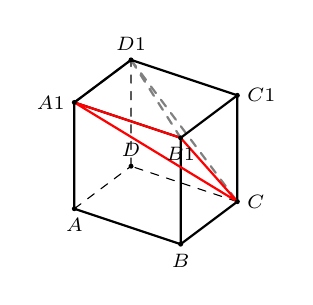
\begin{tikzpicture}[scale=0.9, line join=round, line cap=round]
    \coordinate (A) at (0,0);
    \coordinate (B) at (1.5,-0.5);
    \coordinate (D) at (0.8,0.6);
    \coordinate (C) at (2.3,0.1);
    \coordinate (A1) at (0,1.5);
    \coordinate (B1) at (1.5,1.0);
    \coordinate (D1) at (0.8,2.1);
    \coordinate (C1) at (2.3,1.6);
    \draw[dashed] (A) -- (D) (C) -- (D) (D) -- (D1);
    \draw[dashed, thick, gray] (A1) -- (D1) (D1) -- (C) (B1) -- (D1);
    \draw[thick] (A) -- (B) -- (C) -- (C1) -- (D1) -- (A1) -- cycle;
    \draw[thick] (A1) -- (B1) -- (C1) (B) -- (B1);
    \draw[thick, red] (A1) -- (C) (A1) -- (B1) (B1) -- (C);
    \foreach \p/\pos in {A/below,B/below,C/right,D/above,A1/left,B1/below,C1/right,D1/above} {
      \fill (\p) circle (1.0pt) node[\pos] {\scriptsize \(\p\)};
    }
  \end{tikzpicture}
}
\answerblank[3.5cm]{解：}
\postproblem{
  \item 三棱锥 $A_1-B_1CD_1$ 的四个顶点是否恰好也是正方体的顶点？它们的外接球和正方体的外接球有何关系？
  \item 补形法在此题中是如何把复杂的空间三棱锥模型，瞬间简化为长方体对角线外接球模型的？
}{
  \checkbox 理解了补形法的几何原理 \quad
  \checkbox 掌握了外接球半径模型计算
}{1.2cm}

\newpage

\subsection{专题四：解三角形定理选择与边角互化}

\begin{theorembox}{一、正弦定理与余弦定理选择指南}
遇到三角形问题，根据已知条件的类型快速确定解题路径：
\begin{center}
\arrayrulecolor{rulecolor}
\begin{tabularx}{\textwidth}{p{3.2cm}p{4.0cm}X}
\toprule[1.1pt]
\textbf{已知条件类型} & \textbf{首选定理} & \textbf{公式骨架} \\
\midrule
已知两角及一边 & 正弦定理 & \(\dfrac{a}{\sin A} = \dfrac{b}{\sin B} = \dfrac{c}{\sin C}\) \\ \hline
已知两边及夹角 & 余弦定理 & \(c^2 = a^2 + b^2 - 2ab\cos C\) \\ \hline
已知三边关系 & 余弦定理变式 & \(\cos C = \dfrac{a^2 + b^2 - c^2}{2ab}\) \\ \hline
已知两边及其中一边对角 & 正弦定理 & \(\sin B = \dfrac{b\sin A}{a}\) \\
\bottomrule[1.1pt]
\end{tabularx}
\end{center}
\end{theorembox}

\begin{theorembox}{二、边角互化的两大决策方向}
\begin{enumerate}
  \item \textbf{化角为边（代数路线）}：利用正弦定理 \(a = 2R\sin A\) 将角转换为长度。适合已知条件中含有较多边的乘积或平方和结构。
  \item \textbf{化边为角（三角路线）}：将所有长度化为正弦，利用三角恒等变换（两角和差、二倍角、辅助角公式）化简。适合式子中含有较多内角的正弦、余弦混合加减结构。
\end{enumerate}
\end{theorembox}

\problemheader{经典例题四：边角互化与范围}
{\small 在 \(\triangle ABC\) 中，已知 \(2b\cos C = 2a - c\)，求角 \(B\) 的大小；若 \(b = \sqrt{3}\)，求 \(\triangle ABC\) 面积的最大值。}
\answerblank[4.0cm]{解：}
\postproblem{
  \item 第一问中式子既有边又有角，化边为角还是化角为边更简便？试一试用正弦定理将边化为角。
  \item 第二问在已知 $b$ 和角 $B$ 的情况下，面积 $S = \dfrac{1}{2}ac\sin B$。我们可以联立余弦定理 $b^2 = a^2+c^2-ac\cos B$ 并使用均值不等式求出 $ac$ 的范围吗？
}{
  \checkbox 熟练应用正/余弦定理进行边角互化 \quad
  \checkbox 掌握面积最大值的均值不等式求解
}{1.2cm}

\newpage

\subsection{专题五：卷面表达与规范书写}

\begin{theorembox}{一、大题采分“六步法”}
在解答题的步骤呈现中，必须体现完整的逻辑链条，避免跨步过大被扣步骤分：
\begin{enumerate}
  \item \textbf{设}：清晰定义解题中引入的新变量、几何法建系中的坐标轴及坐标。
  \item \textbf{限}：写出变量的范围或约束（如换元后 $t \geqslant 0$，导数单调区间两端开闭）。
  \item \textbf{联}：写出建立方程的依据定理名称（如“由余弦定理得”，“联立直线与椭圆方程得”）。
  \item \textbf{推}：写出关键变形的逻辑因果词（因为……所以……，等价于……）。
  \item \textbf{算}：呈现关键计算结果（如联立后的判别式 $\Delta$，韦达定理 $x_1+x_2$ 的表达式）。
  \item \textbf{综}：给出最终的文字结论句（如“综上所述，实数 $a$ 的取值范围为……”）。
\end{enumerate}
\end{theorembox}

\begin{theorembox}{二、两大高频表达细节规范}
\begin{itemize}
  \item \textbf{立体几何判定定理“条件组”规范}：\\
  证明线面垂直时，相交线条件必须写齐。标准的四步采分结构为：
  \[
    \text{因为 } 
    \begin{cases}
      b \subset \alpha, c \subset \alpha \\
      b \cap c = P \\
      a \perp b, a \perp c
    \end{cases}
    \text{，所以 } a \perp \alpha.
  \]
  \item \textbf{导数单调性“表格/文字描述”规范}：\\
  求导后必须写齐令 $f'(x) > 0$ 和 $f'(x) < 0$ 的过程，单调区间一律用逗号或文字“和”连接，\textbf{严禁使用并集符号 $\cup$}。
\end{itemize}
\end{theorembox}

\newpage

% =====================================================
% 第四部分：最终式思想与重复本系统训练
% =====================================================
\section{最终式思想与重复本系统训练}

\subsection{最终式思想的定义与核心逻辑}

\mindsetcard{最终式思想}{预判链路，以终为始}{%
  所谓“最终式”，是指题目最终必须出现的、能直接推出目标结论的关键表达式。
  在计算前，对命题逻辑、计算链路和目标形式进行精准预判，从而做到：
  \begin{enumerate}
    \item \textbf{不算也知道怎么算}：看清包装下的核心数学模型与计算终点。
    \item \textbf{知道这样算一定可以}：理清推导与化简的因果链条，保证计算方向的绝对正确。
  \end{enumerate}
}

在实战中，我们通常按照以下五步决策流程来运用最终式思想：
\begin{enumerate}
  \item \textbf{读目标}：明确题目要求的是角、边、比值、范围，还是定值、定点。
  \item \textbf{预测最终式}：预判目标形式，例如求角 $A$ 预测最终式为 $\cos A = \text{常数}$，求比值预测最终式为一元方程等。
  \item \textbf{选择转化工具}：在三角中选择正/余弦定理，在解析几何中选择联立、韦达定理或点差法。
  \item \textbf{压缩运算链路}：跳过繁琐的算术展开，只保留关键的变形步骤与公式骨架。
  \item \textbf{检验目标结构}：确认最终得到的表达式是否已与参数无关，或是否已锁定目标结论。
\end{enumerate}

\subsection{最终式思想在三角函数第一问中的体现}

三角大题的第一问如果难度较高，往往是在“包装”上做文章。最终式思想要求我们从复杂的“包装”中快速识别最终目标，并遵循以下两条核心路径：
\begin{itemize}
  \item \textbf{统一边角与纯边化}：若题目求角或边，第一步应优先将式子中的 $\sin A, \sin B, \sin C$ 利用正弦定理转化为边 $a, b, c$。
  \item \textbf{余弦定理锁定最终式}：将所有的三角函数项化为纯边式后，再使用余弦定理将边长关系翻译为角。例如，将复杂恒等式整理为 $b^2+c^2-a^2 = bc$，即可直接得出 $\cos A = \frac{1}{2}$，从而求得 $A = \frac{\pi}{3}$。
\end{itemize}

\subsection{与解析几何的衔接}

解析几何的压轴题往往运算量巨大，其本质也是“最终式处理”的战场：
\begin{itemize}
  \item \textbf{目标形式暗示计算路径}：定值、定点、定直线等题目中，最终式必然是不含动参的常数或固定关系。这一目标形式倒推我们去设计消元和联立的步骤。
  \item \textbf{运算技巧决定速度，最终式思想决定方向}：在联立与韦达定理展开前，必须知道展开后要整理出怎样的形式（如对称式、齐次式）。如果不清楚最终式的结构，运算极易在中途失控。
\end{itemize}

\subsection{重复本的作用与选题标准}

\begin{keybox}{重复本系统训练法则}
  \textbf{重复本不是普通的错题本}，它的核心作用不是记录错误的答案，而是通过多轮重复建立对流程和计算的熟练感，训练\textbf{“运算链路闪回”}能力——即看到题目，脑海中能瞬间闪回出“先算什么、后算什么、最终算到哪里”的完整计算链路。
\end{keybox}

\textbf{重复本选题标准：}
\begin{enumerate}
  \item \textbf{包装吓人}：表面看似复杂、新颖，但拆开包装后属于常规套路。
  \item \textbf{流程常规但自己不熟}：解题套路已知，但自己动笔时反应较慢或容易卡壳。
  \item \textbf{运算链路长、运算量大}：需要多步变形，易产生计算失误，值得反复训练“算感”。
  \item \textbf{含关键运算技巧}：如分离常数、比值换元、整体换元、消根号等技巧。
\end{enumerate}

\subsection{最终式思想典型方法与技巧}

\begin{theorembox}{方法一：三角纯边化}
  当三角形条件中混合了边与角时，优先使用正弦定理将所有角化为边，构建纯边关系，再使用余弦定理求解。\\
  \textbf{核心链路}：复杂三角式 $\Longrightarrow$ 正弦定理化边 $\Longrightarrow$ 余弦定理识角 $\Longrightarrow$ 得到角或边长关系。
\end{theorembox}

\begin{theorembox}{方法二：分离常数}
  在三角或解析几何中处理复杂分式时，利用分离常数减少变量个数或简化分子。\\
  \textbf{公式模版}：$\dfrac{x-a}{x-b} = 1 + \dfrac{b-a}{x-b}$。在两项相加时，可转化为：
  \[
    \frac{x_1-a}{x_1-b} + \frac{x_2-a}{x_2-b} = 2 + (b-a)\left(\frac{1}{x_1-b} + \frac{1}{x_2-b}\right)
  \]
  配合韦达定理，能极大减少直接通分的运算量。
\end{theorembox}

\begin{theorembox}{方法三：比值换元}
  若题目要求边长比（如 $\frac{b}{c}$）的范围，或者式子中出现齐次结构，可设 $t = \frac{b}{c}$，将多元问题转化为一元函数。\\
  \textbf{经典变形}：利用正弦定理：
  \[
    \frac{b}{c} = \frac{\sin B}{\sin C} = \frac{\sin(A+C)}{\sin C} = \sin A \cot C + \cos A
  \]
  把“边长比”转化为“角函数”求范围。
\end{theorembox}

\begin{theorembox}{方法四：整体换元}
  当题目要求一个复杂的整体表达式（如 $a-c$ 或两个角的差）时，不应拆散硬算，而应直接将目标整体设为一个新变量 $t$ 或 $\theta$，反推关于该变量的一元方程。
\end{theorembox}

\begin{theorembox}{方法五：消根号构造整系数方程}
  若题目中含有整数条件或特定无理数（如特殊的三角函数值），可通过移项、平方逐步消去根号，构造其对应的整系数代数方程。\\
  \textbf{示例}：已知 $x_0 = \cos 75^\circ = \dfrac{\sqrt{6}-\sqrt{2}}{4}$，求关于 $x_0$ 的整系数方程。\\
  解：由 $4x_0 = \sqrt{6}-\sqrt{2}$，两边平方得 $16x_0^2 = 8 - 4\sqrt{3}$，整理得 $4x_0^2 - 2 = -\sqrt{3}$。再次平方得 $(4x_0^2-2)^2 = 3$，即 $16x_0^4 - 16x_0^2 + 1 = 0$。
\end{theorembox}

\begin{theorembox}{方法六：角平分线定理与 Stewart 定理}
  在解三角形中，若涉及角平分线 $AD$，可结合角平分线定理 $\dfrac{BD}{DC} = \dfrac{c}{b}$ 及角平分线长度公式：
  \[
    AD^2 = AB \cdot AC - BD \cdot DC = bc - BD \cdot DC
  \]
  快速建立边长方程。若为一般线段，则使用 Stewart 定理建立关系。
\end{theorembox}

\begin{theorembox}{方法七：正切式整体处理}
  当题目涉及多个角的关系且包含正切值乘积或平方时，引入辅助角。设目标角 $\alpha = \angle AOC$，辅助角 $\beta = \angle BOC$，将其他相关角表示为 $\alpha \pm \beta$，利用正切和差公式：
  \[
    \tan(\alpha+\beta)\tan(\alpha-\beta) = \frac{\tan^2\alpha - \tan^2\beta}{1 - \tan^2\alpha\tan^2\beta}
  \]
  构建含 $\tan^2\alpha$ 和 $\tan^2\beta$ 的方程，再消去辅助变量 $\beta$ 求解目标。
\end{theorembox}

\newpage

% =====================================================
% 第五部分：考场解题思路分析流程图
% =====================================================
\section{考场解题思路分析流程图}

当你在考场上面对一道题目卡壳、算不下去或找不到思路时，请立即启动以下\textbf{解题步骤流程图}进行思维扫描与平移转化：

\vspace{1.0cm}

\begin{center}
  \resizebox{0.95\textwidth}{!}{%
    \begin{tikzpicture}[
      node distance=1.1cm and 1.2cm,
      every node/.style={draw, thick, rectangle, rounded corners=4pt, align=center, inner sep=7pt, fill=white, font=\small},
      arrow/.style={-latex, thick}
    ]
      % Node 1: Stage 1
      \node (stage1) [fill=gray!10, text width=7.5cm] {%
        \textbf{【第一阶段：面对新题】}\\[0.2em]
        立即写出定义域与变量限制条件（定义域优先与边界意识）
      };

      % Node 2: Stage 2 Decision
      \node (stage2) [below=of stage1, fill=gray!5, text width=7.5cm] {%
        \textbf{【第二阶段：双轨路径决策】}\\[0.2em]
        根据题目特征，决定解题突破主路径
      };

      % Branch Left: Geom
      \node (geom) [below left=1.8cm and -0.2cm of stage2, text width=4.8cm] {%
        \textbf{【形之径：图像几何化】}\\[0.3em]
        1. 尝试把代数式画成图像\\[0.2em]
        2. 翻译为斜率、距离或绝对值\\[0.2em]
        3. 寻找几何对称与切线临界
      };

      % Branch Right: Alg
      \node (alg) [below right=1.8cm and -0.2cm of stage2, text width=4.8cm] {%
        \textbf{【数之径：代数结构化】}\\[0.3em]
        1. 寻找超级结构块整体代换\\[0.2em]
        2. 检查变形过程的等价防爆\\[0.2em]
        3. 轴动区间定启动分类讨论
      };

      % Node 3: Stage 3 Check
      \node (stage3) [below=5.0cm of stage2, text width=7.2cm] {%
        \textbf{【第三阶段：临界与边界检验】}\\[0.2em]
        1. 极值点与最值取等条件是否真实存在？\\[0.2em]
        2. 边界等号端点是否需要代回题干验证？
      };

      % Node 4: Stage 4 Write
      \node (stage4) [below=of stage3, fill=gray!10, text width=7.5cm] {%
        \textbf{【第四阶段：规范卷面书写】}\\[0.2em]
        严格按照“设、限、联、推、算、综”六步法\\[0.2em]
        三层书写（公式骨架 + 短逻辑词串联 + 临界解释）
      };

      % Node 5: End
      \node (end) [below=of stage4, fill=black, text=white, text width=4.2cm] {%
        \textbf{规范步骤，完成解答}
      };

      % Connectors
      \draw[arrow] (stage1) -- (stage2);

      \draw[arrow] (stage2.south) -- ++(0,-0.9) -| (geom.north)
        node[pos=0.25, fill=white, inner sep=3pt, font=\small\bfseries] {形之径（几何）};
      \draw[arrow] (stage2.south) -- ++(0,-0.9) -| (alg.north)
        node[pos=0.25, fill=white, inner sep=3pt, font=\small\bfseries] {数之径（代数）};

      \draw[arrow] (geom.south) |- (stage3.west);
      \draw[arrow] (alg.south) |- (stage3.east);

      \draw[arrow] (stage3) -- (stage4);
      \draw[arrow] (stage4) -- (end);
    \end{tikzpicture}%
  }
\end{center}

\end{document}
